\section{Testing}

\subsection{SimpleTest}
\brand{SimpleTest}\footnote{\url{http://simpletest.org/}} ist ein einfaches aber dennoch sehr flexibles Unit Testing Framework.
Die bestehende Funktionalität lässt sich sehr einfach erweitern und auf die eigenen Bedürfnisse anpassen.
Aus diesem Grund sind im Namespace \inlinecode{TestHelper}\footnote{\url{http://kort.herokuapp.com/docs/Kort-backend/namespaces/TestHelper.html}} einige Klassen entstanden als Erweiterung von SimpleTest.
So ist es beispielsweise möglich, die Tests sowohl im Browser, wie auch auf der Kommandozeile auszuführen.

Die Testresultate der Entwicklungsumgebung befinden sich unter \url{http://kort-dev.herokuapp.com/test}.

\begin{figure}[H]
	\centering
	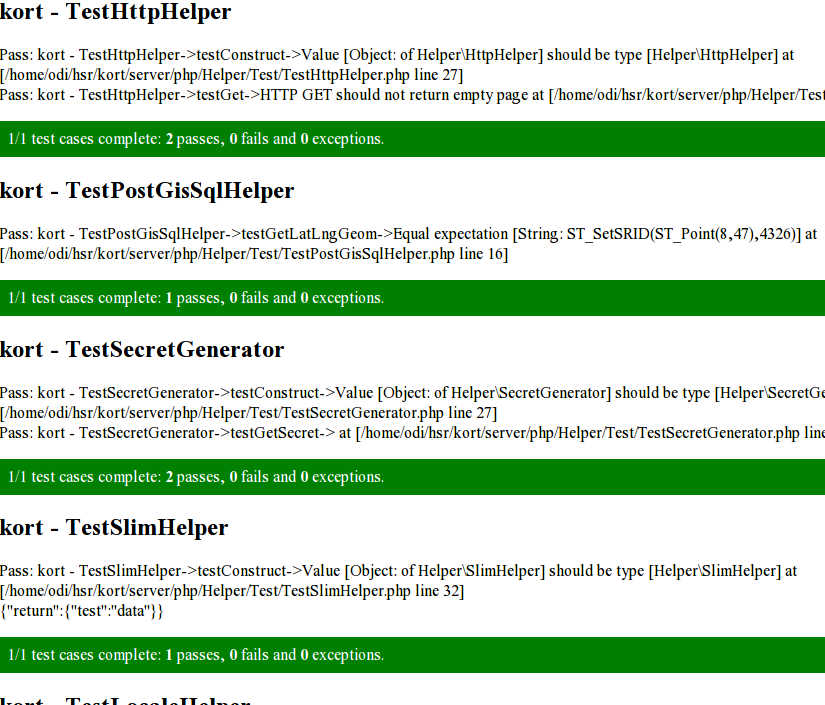
\includegraphics[scale=0.5]{images/implementation/backend/simple-test}
	\caption{Testresultate von SimpleTest im Browser}
	\label{image-simple-test}
\end{figure}

Der derzeitige Build ist so konfiguriert, dass er fehlschlägt, wenn die Tests nicht bestanden werden.
Dies stellt sicher, dass sich nur stabile Versionen auf unserem Webserver befinden.

\subsection{Integrationstests der Webservices mit QUnit}
Neben den klassischen Unit Tests, waren für die verschiedenen \gls{REST}-Webservices auch noch Integrationstest nötig.
Im Rahmen solcher Tests wird via \brand{QUnit} (welches wir für das JavaScript Testing benötigen) eine Anfrage an die betreffende Ressource gestellt.
Deren Antwort lässt sich dann im Unit Test leicht prüfen.

Die JavaScript Tests befinden sich auf der Entwicklungsumgebung unter \url{http://kort-dev.herokuapp.com/test/client/}.

\begin{figure}[H]
	\centering
	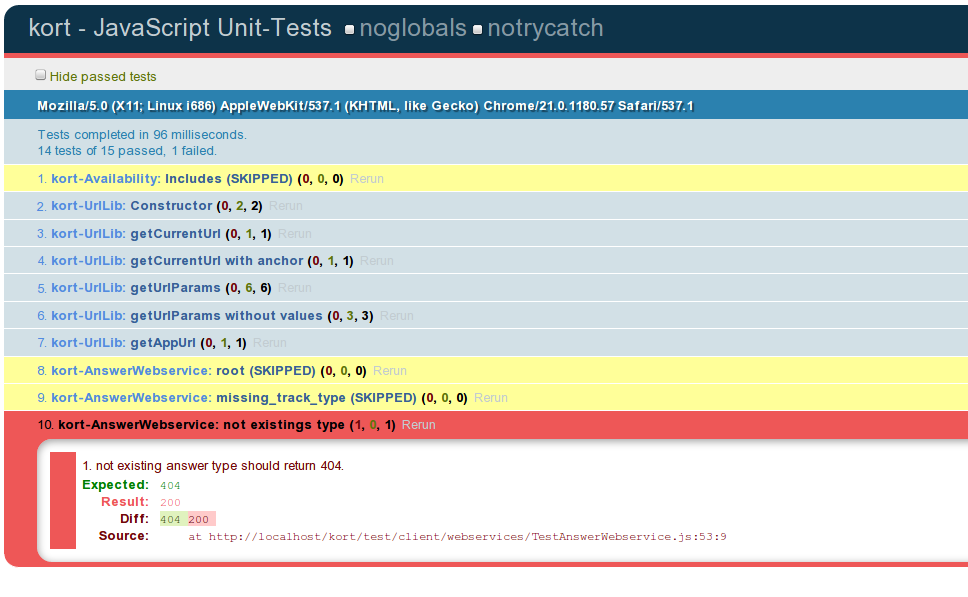
\includegraphics[width=\textwidth]{images/implementation/backend/qunit-skipped-test}
	\caption{Testresultate der Integrationstests im Browser}
	\label{image-qunit-skipped-test}
\end{figure}